%% LyX 2.3.7 created this file.  For more info, see http://www.lyx.org/.
%% Do not edit unless you really know what you are doing.
\documentclass[journal,article,submit,pdftex,moreauthors]{mdpi}
\usepackage[utf8]{inputenc}
\usepackage{float}
\usepackage{url}
\usepackage{graphicx}

\makeatletter

%%%%%%%%%%%%%%%%%%%%%%%%%%%%%% LyX specific LaTeX commands.

\Title{Predict the duration of forestfires using machine learning methods}

\TitleCitation{Predict the duration of forestfires using machine learning methods}

\Author{Constantina Kopitsa$^{1}$, Ioannis G. Tsoulos$^{2*}$, Vasileios
Charilogis$^{3}$, Athanassios Stavrakoudis$^{4}$}

\AuthorNames{Constantina Kopitsa, Ioannis G. Tsoulos, Vasileios Charilogis and
Athanassios Stavrakoudis}

\AuthorCitation{Kopitsa, C.;Tsoulos, I.G.; Charilogis V., Stavrakoudis A.}


\address{$^{1}$\quad{}Department of Informatics and Telecommunications,
University of Ioannina, Greece;k.kopitsa@uoi.gr\\
$^{2}$\quad{}Department of Informatics and Telecommunications, University
of Ioannina, Greece; itsoulos@uoi.gr\\
$^{3}\quad$Department of Informatics and Telecommunications, University
of Ioannina, Greece; v.charilog@uoi.gr\\
$^{4}\quad$Department of Economics, University of Ioannina, Ioannina,
Greece; astavrak@uoi.gr}


\corres{Correspondence: itsoulos@uoi.gr}


\abstract{Forest and urban fires are a major problem in the modern era that
tests the endurance of governments to extinguish them. Fires can cause
economic and ecological problems especially in the summer months.
In modern times, the rapid development of Artificial Intelligence
can be a weapon for predicting the evolution of fires or even for
their prevention. Specifically, through Machine Learning, which is
one part of Artificial Intelligence several methods have been incorporated
to detect the duration of fires using data which are freely available
from the Fire Service of Greece for a period of 10 years.\textbf{
}For this purpose, a wide range of machine learning techniques were
used on this data and the experimental results were more than encouraging.}


\keyword{Forest fires; Machine learning; Neural networks; Decision trees}

\DeclareTextSymbolDefault{\textquotedbl}{T1}
%% Because html converters don't know tabularnewline
\providecommand{\tabularnewline}{\\}

%%%%%%%%%%%%%%%%%%%%%%%%%%%%%% User specified LaTeX commands.
%  LaTeX support: latex@mdpi.com 
%  For support, please attach all files needed for compiling as well as the log file, and specify your operating system, LaTeX version, and LaTeX editor.

%=================================================================


% For posting an early version of this manuscript as a preprint, you may use "preprints" as the journal and change "submit" to "accept". The document class line would be, e.g., \documentclass[preprints,article,accept,moreauthors,pdftex]{mdpi}. This is especially recommended for submission to arXiv, where line numbers should be removed before posting. For preprints.org, the editorial staff will make this change immediately prior to posting.

%--------------------
% Class Options:
%--------------------
%----------
% journal
%----------
% Choose between the following MDPI journals:
% acoustics, actuators, addictions, admsci, adolescents, aerospace, agriculture, agriengineering, agronomy, ai, algorithms, allergies, alloys, analytica, animals, antibiotics, antibodies, antioxidants, applbiosci, appliedchem, appliedmath, applmech, applmicrobiol, applnano, applsci, aquacj, architecture, arts, asc, asi, astronomy, atmosphere, atoms, audiolres, automation, axioms, bacteria, batteries, bdcc, behavsci, beverages, biochem, bioengineering, biologics, biology, biomass, biomechanics, biomed, biomedicines, biomedinformatics, biomimetics, biomolecules, biophysica, biosensors, biotech, birds, bloods, blsf, brainsci, breath, buildings, businesses, cancers, carbon, cardiogenetics, catalysts, cells, ceramics, challenges, chemengineering, chemistry, chemosensors, chemproc, children, chips, cimb, civileng, cleantechnol, climate, clinpract, clockssleep, cmd, coasts, coatings, colloids, colorants, commodities, compounds, computation, computers, condensedmatter, conservation, constrmater, cosmetics, covid, crops, cryptography, crystals, csmf, ctn, curroncol, currophthalmol, cyber, dairy, data, dentistry, dermato, dermatopathology, designs, diabetology, diagnostics, dietetics, digital, disabilities, diseases, diversity, dna, drones, dynamics, earth, ebj, ecologies, econometrics, economies, education, ejihpe, electricity, electrochem, electronicmat, electronics, encyclopedia, endocrines, energies, eng, engproc, ent, entomology, entropy, environments, environsciproc, epidemiologia, epigenomes, est, fermentation, fibers, fintech, fire, fishes, fluids, foods, forecasting, forensicsci, forests, foundations, fractalfract, fuels, futureinternet, futureparasites, futurepharmacol, futurephys, futuretransp, galaxies, games, gases, gastroent, gastrointestdisord, gels, genealogy, genes, geographies, geohazards, geomatics, geosciences, geotechnics, geriatrics, hazardousmatters, healthcare, hearts, hemato, heritage, highthroughput, histories, horticulturae, humanities, humans, hydrobiology, hydrogen, hydrology, hygiene, idr, ijerph, ijfs, ijgi, ijms, ijns, ijtm, ijtpp, immuno, informatics, information, infrastructures, inorganics, insects, instruments, inventions, iot, j, jal, jcdd, jcm, jcp, jcs, jdb, jeta, jfb, jfmk, jimaging, jintelligence, jlpea, jmmp, jmp, jmse, jne, jnt, jof, joitmc, jor, journalmedia, jox, jpm, jrfm, jsan, jtaer, jzbg, kidney, kidneydial, knowledge, land, languages, laws, life, liquids, literature, livers, logics, logistics, lubricants, lymphatics, machines, macromol, magnetism, magnetochemistry, make, marinedrugs, materials, materproc, mathematics, mca, measurements, medicina, medicines, medsci, membranes, merits, metabolites, metals, meteorology, methane, metrology, micro, microarrays, microbiolres, micromachines, microorganisms, microplastics, minerals, mining, modelling, molbank, molecules, mps, msf, mti, muscles, nanoenergyadv, nanomanufacturing, nanomaterials, ncrna, network, neuroglia, neurolint, neurosci, nitrogen, notspecified, nri, nursrep, nutraceuticals, nutrients, obesities, oceans, ohbm, onco, oncopathology, optics, oral, organics, organoids, osteology, oxygen, parasites, parasitologia, particles, pathogens, pathophysiology, pediatrrep, pharmaceuticals, pharmaceutics, pharmacoepidemiology, pharmacy, philosophies, photochem, photonics, phycology, physchem, physics, physiologia, plants, plasma, pollutants, polymers, polysaccharides, poultry, powders, preprints, proceedings, processes, prosthesis, proteomes, psf, psych, psychiatryint, psychoactives, publications, quantumrep, quaternary, qubs, radiation, reactions, recycling, regeneration, religions, remotesensing, reports, reprodmed, resources, rheumato, risks, robotics, ruminants, safety, sci, scipharm, seeds, sensors, separations, sexes, signals, sinusitis, skins, smartcities, sna, societies, socsci, software, soilsystems, solar, solids, sports, standards, stats, stresses, surfaces, surgeries, suschem, sustainability, symmetry, synbio, systems, taxonomy, technologies, telecom, test, textiles, thalassrep, thermo, tomography, tourismhosp, toxics, toxins, transplantology, transportation, traumacare, traumas, tropicalmed, universe, urbansci, uro, vaccines, vehicles, venereology, vetsci, vibration, viruses, vision, waste, water, wem, wevj, wind, women, world, youth, zoonoticdis 

%---------
% article
%---------
% The default type of manuscript is "article", but can be replaced by: 
% abstract, addendum, article, book, bookreview, briefreport, casereport, comment, commentary, communication, conferenceproceedings, correction, conferencereport, entry, expressionofconcern, extendedabstract, datadescriptor, editorial, essay, erratum, hypothesis, interestingimage, obituary, opinion, projectreport, reply, retraction, review, perspective, protocol, shortnote, studyprotocol, systematicreview, supfile, technicalnote, viewpoint, guidelines, registeredreport, tutorial
% supfile = supplementary materials

%----------
% submit
%----------
% The class option "submit" will be changed to "accept" by the Editorial Office when the paper is accepted. This will only make changes to the frontpage (e.g., the logo of the journal will get visible), the headings, and the copyright information. Also, line numbering will be removed. Journal info and pagination for accepted papers will also be assigned by the Editorial Office.

%------------------
% moreauthors
%------------------
% If there is only one author the class option oneauthor should be used. Otherwise use the class option moreauthors.

%---------
% pdftex
%---------
% The option pdftex is for use with pdfLaTeX. If eps figures are used, remove the option pdftex and use LaTeX and dvi2pdf.

%=================================================================
% MDPI internal commands - do not modify
\firstpage{1} 
 
\setcounter{page}{\@firstpage} 

\pubvolume{1}
\issuenum{1}
\articlenumber{0}
\pubyear{2024}
\copyrightyear{2024}
%\externaleditor{Academic Editor: Firstname Lastname} % For journal Automation, please change Academic Editor to "Communicated by"
\datereceived{}
\daterevised{ } % Comment out if no revised date
\dateaccepted{}
\datepublished{}
%\datecorrected{} % Corrected papers include a "Corrected: XXX" date in the original paper.
%\dateretracted{} % Corrected papers include a "Retracted: XXX" date in the original paper.
\hreflink{https://doi.org/} % If needed use \linebreak
%\doinum{}
%------------------------------------------------------------------
% The following line should be uncommented if the LaTeX file is uploaded to arXiv.org
%\pdfoutput=1

%=================================================================
% Add packages and commands here. The following packages are loaded in our class file: fontenc, inputenc, calc, indentfirst, fancyhdr, graphicx, epstopdf, lastpage, ifthen, lineno, float, amsmath, setspace, enumitem, mathpazo, booktabs, titlesec, etoolbox, tabto, xcolor, soul, multirow, microtype, tikz, totcount, changepage, attrib, upgreek, cleveref, amsthm, hyphenat, natbib, hyperref, footmisc, url, geometry, newfloat, caption

%=================================================================
%% Please use the following mathematics environments: Theorem, Lemma, Corollary, Proposition, Characterization, Property, Problem, Example, ExamplesandDefinitions, Hypothesis, Remark, Definition, Notation, Assumption
%% For proofs, please use the proof environment (the amsthm package is loaded by the MDPI class).

%=================================================================
% The fields PACS, MSC, and JEL may be left empty or commented out if not applicable
%\PACS{J0101}
%\MSC{}
%\JEL{}

%%%%%%%%%%%%%%%%%%%%%%%%%%%%%%%%%%%%%%%%%%
% Only for the journal Diversity
%\LSID{\url{http://}}

%%%%%%%%%%%%%%%%%%%%%%%%%%%%%%%%%%%%%%%%%%
% Only for the journal Applied Sciences:
%\featuredapplication{Authors are encouraged to provide a concise description of the specific application or a potential application of the work. This section is not mandatory.}
%%%%%%%%%%%%%%%%%%%%%%%%%%%%%%%%%%%%%%%%%%

%%%%%%%%%%%%%%%%%%%%%%%%%%%%%%%%%%%%%%%%%%
% Only for the journal Data:
%\dataset{DOI number or link to the deposited data set in cases where the data set is published or set to be published separately. If the data set is submitted and will be published as a supplement to this paper in the journal Data, this field will be filled by the editors of the journal. In this case, please make sure to submit the data set as a supplement when entering your manuscript into our manuscript editorial system.}

%\datasetlicense{license under which the data set is made available (CC0, CC-BY, CC-BY-SA, CC-BY-NC, etc.)}

%%%%%%%%%%%%%%%%%%%%%%%%%%%%%%%%%%%%%%%%%%
% Only for the journal Toxins
%\keycontribution{The breakthroughs or highlights of the manuscript. Authors can write one or two sentences to describe the most important part of the paper.}

%%%%%%%%%%%%%%%%%%%%%%%%%%%%%%%%%%%%%%%%%%
% Only for the journal Encyclopedia
%\encyclopediadef{Instead of the abstract}
%\entrylink{The Link to this entry published on the encyclopedia platform.}
%%%%%%%%%%%%%%%%%%%%%%%%%%%%%%%%%%%%%%%%%%

%%%%%%%%%%%%%%%%%%%%%%%%%%%%%%%%%%%%%%%%%%
% Only for the journal Advances in Respiratory Medicine
%\addhighlights{yes}
%\renewcommand{\addhighlights}{%

%\noindent This is an obligatory section in “Advances in Respiratory Medicine”, whose goal is to increase the discoverability and readability of the article via search engines and other scholars. Highlights should not be a copy of the abstract, but a simple text allowing the reader to quickly and simplified find out what the article is about and what can be cited from it. Each of these parts should be devoted up to 2~bullet points.\vspace{3pt}\\
%\textbf{What are the main findings?}
% \begin{itemize}[labelsep=2.5mm,topsep=-3pt]
% \item First bullet.
% \item Second bullet.
% \end{itemize}\vspace{3pt}
%\textbf{What is the implication of the main finding?}
% \begin{itemize}[labelsep=2.5mm,topsep=-3pt]
% \item First bullet.
% \item Second bullet.
% \end{itemize}
%}
%%%%%%%%%%%%%%%%%%%%%%%%%%%%%%%%%%%%%%%%%%

\makeatother

\begin{document}
\maketitle

\section{Introduction}

Forests play an important role in the ecological balance \citep{forest1}
of our planet as well as in our everyday life \citep{forest2}. However,
these ecosystems are threatened by various risks, the most important
of which are fires \citep{fire1,fire2,fire3}. Forest fires destroy
the forest ecosystem \citep{fire_eco1,fire_eco2,fire_eco3} and can
have devastating effects on local economies \citep{fire_econ1,fire_econ2},
with a significant impact also on tourism development \citep{fire_tourism1,fire_tourism2,fire_tourism3}
as well as in human health \citep{fire_health1,fire_health2,fire_health3}. 

Since the risks of fires are great, governments must take measures
and review them in the direction of fire prevention by analyzing data
collected from fires that have broken out in recent history \citep{fire_stat1,fire_stat2,fire_stat3}.
Also, local authorities have used techniques for forest fire monitoring,
such as small UAVs \citep{fire_monitor1}, usage of a monitoring system
based on GPRS and ZigBee wireless network \citep{fire_monitor2},
the iForestFire system \citep{fire_monitor3} etc. Merino et al. suggested
an Unmanned Aircraft System (UAS) \citep{fire_monitor4} for forest
fire monitoring. Also, Aslan et al. proposed a system \citep{fire_monitor5}
of wireless sensor networks for forest fire detection and monitoring.
Recently, Serna et al. suggested a distributed system for fire monitoring
using wireless sensor networks \citep{fire_monitor6}. 

During recent years, machine learning techniques have started to play
an important role in the prevention and treatment of forest fires.
For example, Dwiasnati and Devianto proposed the usage of various
machine learning methods for the classification of forest fire areas
\citep{fire_area_class}. Also, Pang et al. suggested the usage of
a series of machine learning models to forest fire occurrence prediction
in China \citep{fire_prediction_china}. Dampage et al. suggested
a system of wireless sensor networks with data handled by machine
learning models for the detection of forest fires \citep{fire_detection_dampage}.
Shao et al. proposed a mapping of China's forest fire risks using
a series of machine learning models \citep{fire_risk}. A parallel
SVM model is also suggested by Singh et al. \citep{fire_parallel_svm}
for forest fire prediction on data collected from India and Portugal.
A survey on machine learning models used for forest fire prediction
can be found in the work of Abid \citep{fire_ml_survey}. 

In addition, image processing has been established as a fire detection
method. In this direction, a multitude of techniques have been presented
that also take advantage of machine learning methods, such as the
work of Vicente and Guillemant that presented a method for early smoke
source detection \citep{fire_image1}. Also, Yan et al. proposed a
method \citep{fire_image2} that combined image processing techniques
and neural networks for forest fire recognition. Mubarak et al. suggested
a rule - based image processing algorithm \citep{fire_image4} for
forest fire detection. Convolution neural networks were utilized in
the work of Wang et al. \citep{fire_image5} for forest fire image
recognition. Also, wavelet analysis was used in the work of Jiao et
al. \citep{fire_image6} for forest fire detection.

This research work focuses on the use of machine learning techniques
to predict the duration of forest fires, which occurred in Greece
from 2014 until 2023. The data was collected by the Hellenic Fire
Service and then, after clearing missing records, the data was digitized
and one of three categories was assigned to every pattern: fires of
short duration, fires of medium duration and fires of long duration.
The prediction of the duration of a fire is important as in this way,
on the one hand, an estimate can be made of the expected damage that
will be caused in the area, and on the other, the human resources
required to extinguish the fire can be calculated. Similar works in
this area include the work of Liang et al. that used the duration
of a wildfire and the burnt area to determine the scale of wildfires
using neural networks \citep{fire_duration1}. Also, KC et al.. proposed
a Surrogate model \citep{fire_duration2} to model the size of a wildfire
over time, using data collected from wildfires in Tasmania. Furthermore,
Xi et al. proposed \citep{fire_duration3} the application of joint
mixture models to model the duration and the size of wildfires.

The rest of this article is divided as follows: in section \ref{sec:Materials-and-Methods}
the used dataset is described as well as the incorporated machine
learning methods, in section \ref{sec:Results} the experimental results
are fully described and finally in section \ref{sec:Conclusions}
some conclusions are discussed accompanied by some guidelines for
future research.

\section{Materials and Methods\label{sec:Materials-and-Methods}}

This section presents the datasets that will be used in the experiments
as well as the machine learning techniques that will be applied to
these datasets. 

\subsection{The used datasets}

In this research work, open data was used which is available from
the Hellenic Fire Service at the relevant link \url{https://www.fireservice.gr/en_US/synola-dedomenon}(accessed
on 14 September 2024). The data was obtained for the years 2014-2023
and data preprocessing techniques were applied before inputting the
data into machine learning models.

The initial datasets contain information in both numerical and alphanumeric
form, such as the area in which the forest fire occurred or the fire
station that extinguished it. Therefore, the first step in preprocessing
the data was to digitize the columns that contained numerical information
and replace them with a discrete integer. The next important step
in the preprocessing of the original data is to delete the records
that contain empty values in various attributes. This could happen,
for example, if a value was not available at the time of entry. Those
records in which the duration of the fire was zero were also deleted.
Then, to create the exit category, the duration of the forest fire
was converted into minutes. In order to address highly skewed and
non-normal distribution of the dependent variable (fire duration)
we used the commonly applied method of natural log transformation
for minutes. This allowed the variance stabilization of the dependent
variable and transformed its distribution much closer to normal, allowing
a better allowance for linear modeling and greatly reducing the impact
of outliers\textbf{ }\citep{log_norm}. Subsequently, three distinct
values were created depending on the logarithmic value of the duration
in minutes of the forest fire: one value is used for short duration
forest fires, one distinct class for forest fires of medium duration
and one class for the forest fires with long duration.\textbf{ }This
value will be used as the target value in running the experiments.
The preprocessing steps are graphically illustrated in Figure \ref{fig:preSteps}.

\begin{figure}[H]
\begin{centering}
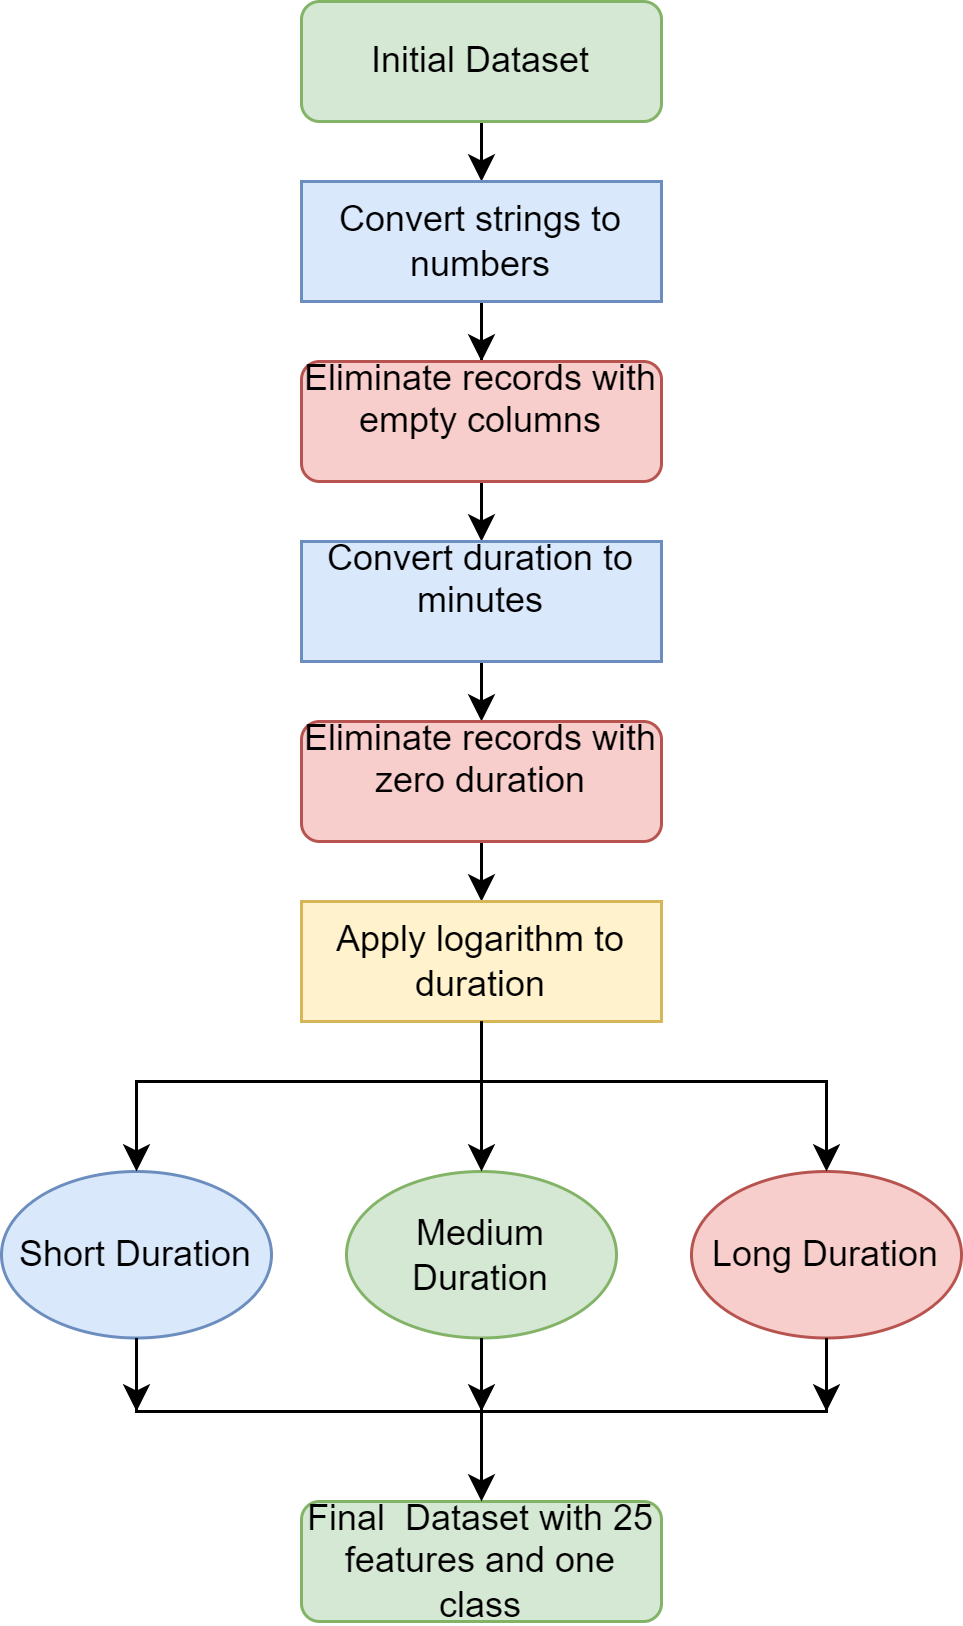
\includegraphics[scale=0.4]{forest_diagram}
\par\end{centering}
\caption{The steps of the preprocessing that were applied on the original datasets.\label{fig:preSteps}}

\end{figure}

Having performed the previously mentioned preprocessing steps, the
final datasets contain 25 features and the following information about
the forest fires:
\begin{enumerate}
\item Fire department. 
\item Province.
\item Season.
\item Burnt area: forest area, grove, grasslands, reeds/swamps, agricultural
lands, cover crop, garbage dumps.
\item Personnel: Firefighters, volunteers, army, etc. 
\item Vehicles: firefighting, tanks, etc.
\item Aerial means: helicopters, different aircrafts. 
\end{enumerate}

\subsection{The used machine learning methods}

A number of machine learning techniques were used to efficiently find
classes in the datasets of the previous subsection. These techniques
cover a wide range of techniques available in the field of machine
learning and are presented in more detail below. 

\subsubsection{Bayesian Networks}

Bayesian networks are probabilistic models based on direct acyclic
graphs \citep{bayes_net1,bayes_net2} and they have been applied with
success in various cases. For example, Friedman et al. used Bayesian
Networks to analyze expression data \citep{bayes_net_expression}.
Also, Cai et al. used Bayesian Networks in fault diagnosis \citep{bayes_net_fault}
and Barton et al. proposed the use of Bayesian Networks to environmental
problems \citep{bayes_net_environ}. In the case of forest fires,
Bayesian Networks have been used in many cases, such as to predict
and analyze possible fire causes \citep{bayes_net_fire_cause}. The
study was conducted in Mugla of Turkey. Also, Bayesian networks were
used to model the cascading impacts of drought and forest fire in
a recent study \citep{bayes_net_cascade}. Also, Bayesian Networks
were combined with deep learning for detection of fires from video
frames \citep{bayes_net_video}.

\subsubsection{Naïve Bayes }

The Naïve Bayes is a supervised machine learning algorithm, used for
classification tasks. This classifier, uses principles of probability
in order to perform classification tasks \citep{naive_bayes1,naive_bayes2}.
This algorithm has been incorporated in many research areas, such
as document classification \citep{naive_bayes_document}, traffic
risk management \citep{naive_bayes_traffic}, network intrusion detection
\citep{naive_bayes_network} etc. Also, the Naive Bayes has been used
in forest fire issues in a series of papers. For example, Nugroho
et al. proposed a system for forest fire prevention using a combination
of a wireless sensor network and a Naïve Bayes classifier \citep{naive_bayes_fire1}.
A classification of hotspots causing forest fires using the Naive
Bayes algorithm is proposed in the work of Zainul et al. \citep{naive_bayes_fire2}.
Karo et al. proposed a methodology to classify wildfires using feature
selection and the Naive Bayes among other machine learning methods
\citep{naive_bayes_fire3}. Also, a variant of the Naïve Bayes Algorith
was suggested by Shu et al. for forest fire prediction \citep{naive_bayes_fire4}. 

\subsubsection{Logistic Regression}

Like the previously mentioned algorithms, Logistic Regression, works
also with machine learning classification and it can be considered
as a data analysis technique used to predict probabilities \citep{logistic_def}.
Cabrera proposed the Logistic Regression for higher school decisions
\citep{logistic_education}. Also, Lawson et al. proposed the usage
of Logistic Regression method to analyze customer satisfaction data
\citep{logistic_customer}. Hu and Lo used the Logistic Regression
technique to model urban growth in their paper \citep{logistic_urban}.
This method has been used also in a series of issues involving forest
fires, such as human - caused wildfire risk estimation \citep{logistic_fire1},
prediction of wildfire vulnerability \citep{logistic_fire2}, probabilistic
modeling of wildfire occurrence \citep{logistic_fire3}, analysis
of wildfire danger \citep{logistic_fire4}etc.

\subsubsection{Artificial neural networks }

Artificial neural networks (ANNs) are parametric models \citep{nn1,nn2},
where a set of parameters, commonly called weights, must be calculated
to be adapted to classification or regression data. This machine learning
model has been utilized in a variety of scientific and real - world
problems, such as physics problems \citep{nnphysics1,nnphysics2,nnphysics3},
solving differential equations \citep{nnde1,nnde2}, solar radiation
prediction \citep{nn_solar}, agriculture problems \citep{nnagr1,nnagr2},
problems appeared in chemistry \citep{nnchem1,nnchem2,nnchem3}, wind
speed forecasting \citep{nn_wind}, economics problems \citep{nnecon1,nnecon2,nncecon3},
problems related to medicine \citep{nnmed1,nnmed2} etc.

In the area of forest fire prediction and observation, a number of
works using artificial neural networks have been published. Hossain
et al. used ANNs to detect flames and smoke from static image features
\citep{nn_fire1}. Lall and Mathibela utilized neural networks to
predict the risk of wildfires in the city of Cape Town \citep{nn_fire2}.
Also, Sayad et al. used neural networks among other machine learning
techniques for predictive modeling of wildfires from data collected
from NASA's Land Processes Distributed Active Archive Center (LP DAAC)
\citep{nn_fire3}. Artificial neural networks and meteorological data
were used in the work of Liang et al. to predict the scale of wildfires
\citep{nn_fire4}. Also, a case study for predicting wildfires for
a Chinese province using neural networks was published recently by
Gao et al. \citep{nn_fire5}. 

\subsubsection{The J48 algorithm }

The J48 algorithm \citep{j48_1} is one of the most used supervised
machine learning algorithms, used to construct decision trees for
classification data. This method was tested on a series of classification
problems, such as prediction of diabetes \citep{j48_diabetes}, network
intrusion detection \citep{j48_network}, classification of criminal
data \citep{j48_criminal}, fingerprint gender classification \citep{j48_finger},
fake news classification \citep{j48_fake} etc. Also, the J48 algorithm
was used to predict forest fires using data from Slovenia in a recent
work \citep{j48_forest2}. A similar study was performed in Algeria
using the J48 algorithm among other machine learning models \citep{j48_forest2}.

\subsubsection{Random Forests}

Random Forest \citep{random_forest1,random_forest2} is a popular
supervised machine learning algorithm, used to construct decision
trees for classification problems. The method of Random Forests has
proven its adaptability and effectiveness in a number of difficult
problems, such as remote sensing classification \citep{random_forest_remote},
ecology issues \citep{random_forest_ecology}, bionformatics \citep{random_forest_bio},
text categorization \citep{random_forest_text}, network intrusion
detection \citep{random_forest_network} etc. Moreover, random forest
was incorporated for forest fire prediction, such as in the work of
Latifah et al., where random forests were applied to predict forest
fires in Borneo \citep{random_forest_fire1}. Also, Malik et al. proposed
the usage of Random Forests for wildfire risk prediction in Northern
California \citep{random_forest_fire2}. Also, Gao et al. performed
a forest fire risk prediction \citep{random_forest_fire3} in China
using a combination of Random Forests and a neural network trained
with the Back Propagation method \citep{bpnn1}.

\section{Results\label{sec:Results}}

The experiments were conducted using the freely available programming
tool of WEKA \citep{weka_main}. The software, which is written in
the JAVA programming language to be portable, can be downloaded freely
from \url{https://ml.cms.waikato.ac.nz/weka/}(accessed on 14 September
2024) or it can be found in the repositories of most Linux systems.
The WEKA software is a collection of machine learning and data analysis
tools and it contains also some visualization tools for modeling.
The WEKA has been used with success in many cases, such as educational
problems \citep{weka_education1,weka_education2}, medical problems
\citep{weka_medical1,weka_medical2} etc. The validation of the conducted
experiments was performed using the ten - fold cross validation technique.
 The experiments were carried out on an AMD Ryzen 5950X with 128GB
of RAM, running the Debian Linux operating system. The experimental
results using the methods mentioned in the previous section and the
10 modified datasets from the Hellenic Fire Service are listed in
Table \ref{tab:experResults}. The following applies to the tables
of experimental results:
\begin{enumerate}
\item The numbers in cells denote average classification error as calculated
on the test set.
\item The column YEAR denotes the year where the machine learning methods
were applied.
\item The column BAYESNET stands for the application of the Bayesian Network
method.
\item The column NAIVEBAYES denotes the application of the Naïve Bayes algorithm.
\item The column LOGISTIC represents the application of the Logistic Regression
algorithm.
\item The column MLP denotes the application of a neural network to the
dataset.
\item The column J48 denotes the application of the J48 method to the forest
fire data.
\item The column RANDOMFOREST denotes the usage of the Random Forest method
to the data.
\item The row AVERAGE denotes the average classification error for all datasets.
\end{enumerate}
\begin{table}[H]
\caption{Experimental results using various machine learning models for 10
years of observations. The numbers in cells denote average classification
error as measured on the test set.\label{tab:experResults}}

\centering{}%
\begin{tabular}{|c|c|c|c|c|c|c|}
\hline 
\textbf{\footnotesize{}YEAR} & \textbf{\footnotesize{}BAYESNET} & \textbf{\footnotesize{}NAIVEBAYES} & \textbf{\footnotesize{}LOGISTIC} & \textbf{\footnotesize{}MLP} & \textbf{\footnotesize{}J48} & \textbf{\footnotesize{}RANDOMFOREST}\tabularnewline
\hline 
\hline 
2014 & 11.44\% & 12.89\% & 9.81\% & 11.37\% & 10.04\% & 9.42\%\tabularnewline
\hline 
2015 & 11.08\% & 11.26\% & 9.53\% & 10.65\% & 9.51\% & 8.95\%\tabularnewline
\hline 
2016 & 25.71\% & 13.00\% & 3.41\% & 3.90\% & 3.65\% & 3.00\%\tabularnewline
\hline 
2017 & 11.04\% & 11.51\% & 9.48\% & 10.08\% & 10.30\% & 9.29\%\tabularnewline
\hline 
2018 & 11.20\% & 10.46\% & 9.09\% & 9.48\% & 9.27\% & 8.58\%\tabularnewline
\hline 
2019 & 9.61\% & 9.25\% & 8.29\% & 8.53\% & 9.08\% & 8.01\%\tabularnewline
\hline 
2020 & 18.00\% & 6.72\% & 5.54\% & 5.97\% & 6.09\% & 5.50\%\tabularnewline
\hline 
2021 & 12.35\% & 14.15\% & 12.04\% & 13.59\% & 13.59\% & 11.92\%\tabularnewline
\hline 
2022 & 10.25\% & 9.62\% & 9.01\% & 9.47\% & 9.04\% & 8.93\%\tabularnewline
\hline 
2023 & 9.74\% & 9.19\% & 8.26\% & 8.77\% & 8.39\% & 7.66\%\tabularnewline
\hline 
\textbf{AVERAGE} & \textbf{13.04\%} & \textbf{10.81\%} & \textbf{8.45\%} & \textbf{9.18\%} & \textbf{8.90\%} & \textbf{8.13\%}\tabularnewline
\hline 
\end{tabular}
\end{table}
Judging from the experimental results it is evident that the Random
Forest technique excellently outweighs the others along with the Logistic
Regression technique. This observations is reinforced from  the box
plot of Figure \ref{fig:boxPlot}. 

\begin{figure}[H]
\begin{centering}
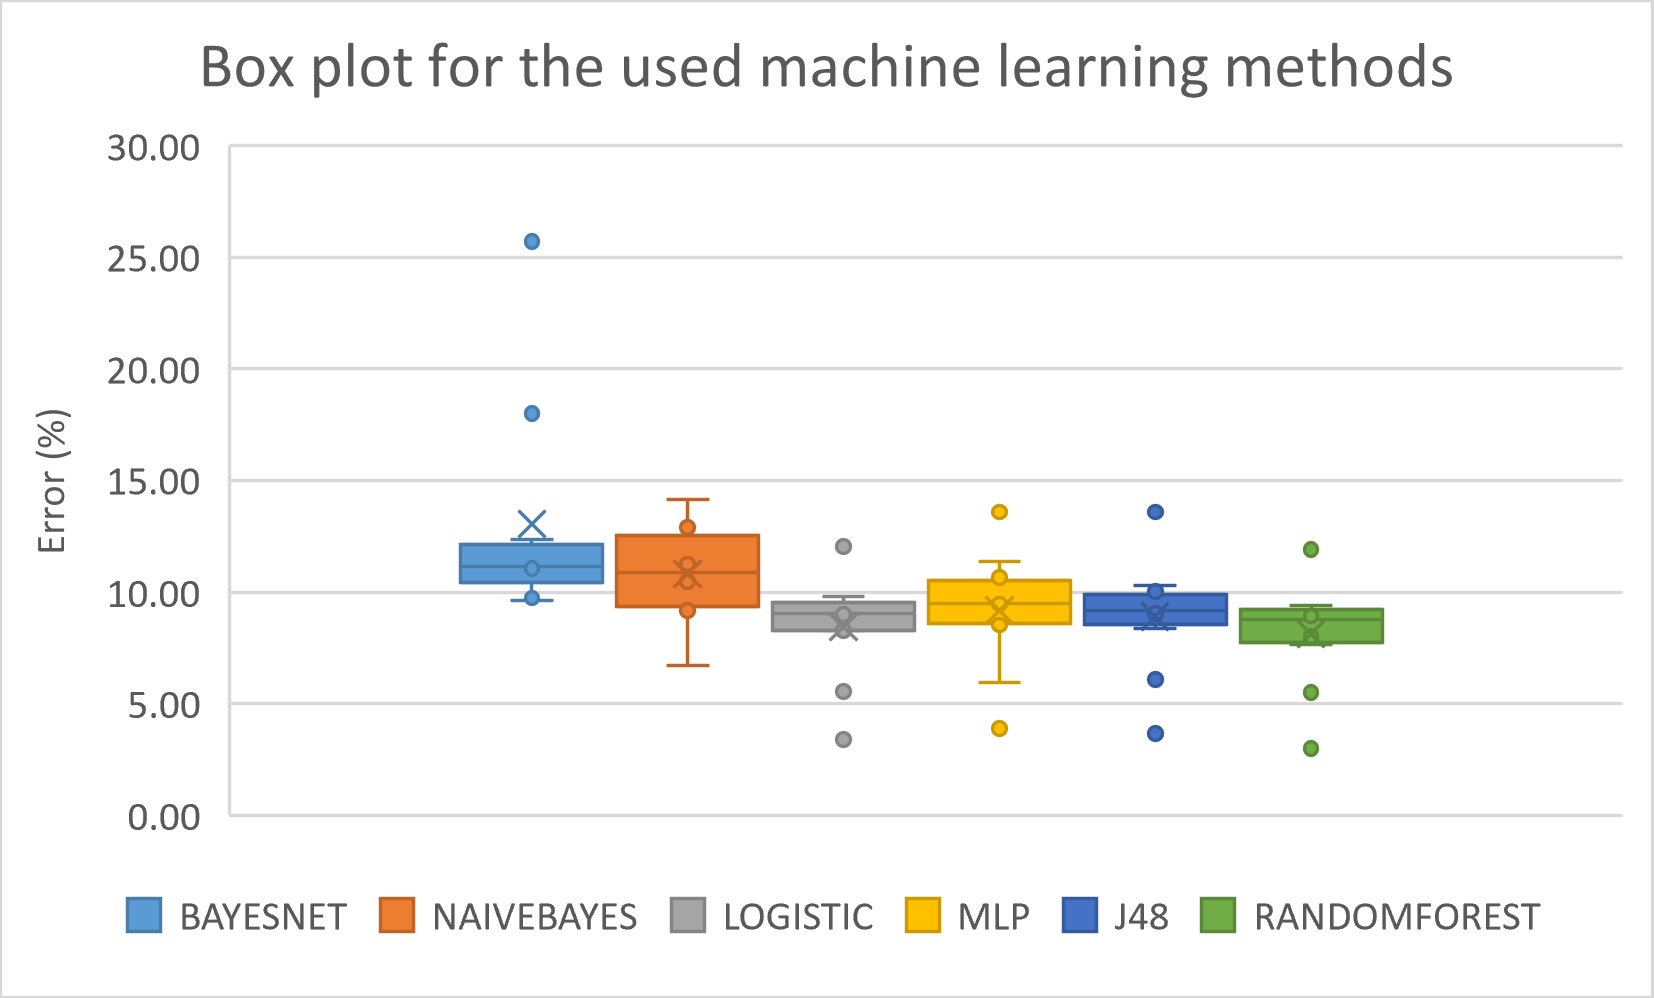
\includegraphics{boxplot}
\par\end{centering}
\caption{Box plot for the used machine learning techniques. \label{fig:boxPlot}}

\end{figure}
The statistical comparison of the Random Forest with the other machine
learning methods is depicted in Figure \ref{fig:statRandomForest}.
\begin{figure}[H]
\begin{centering}
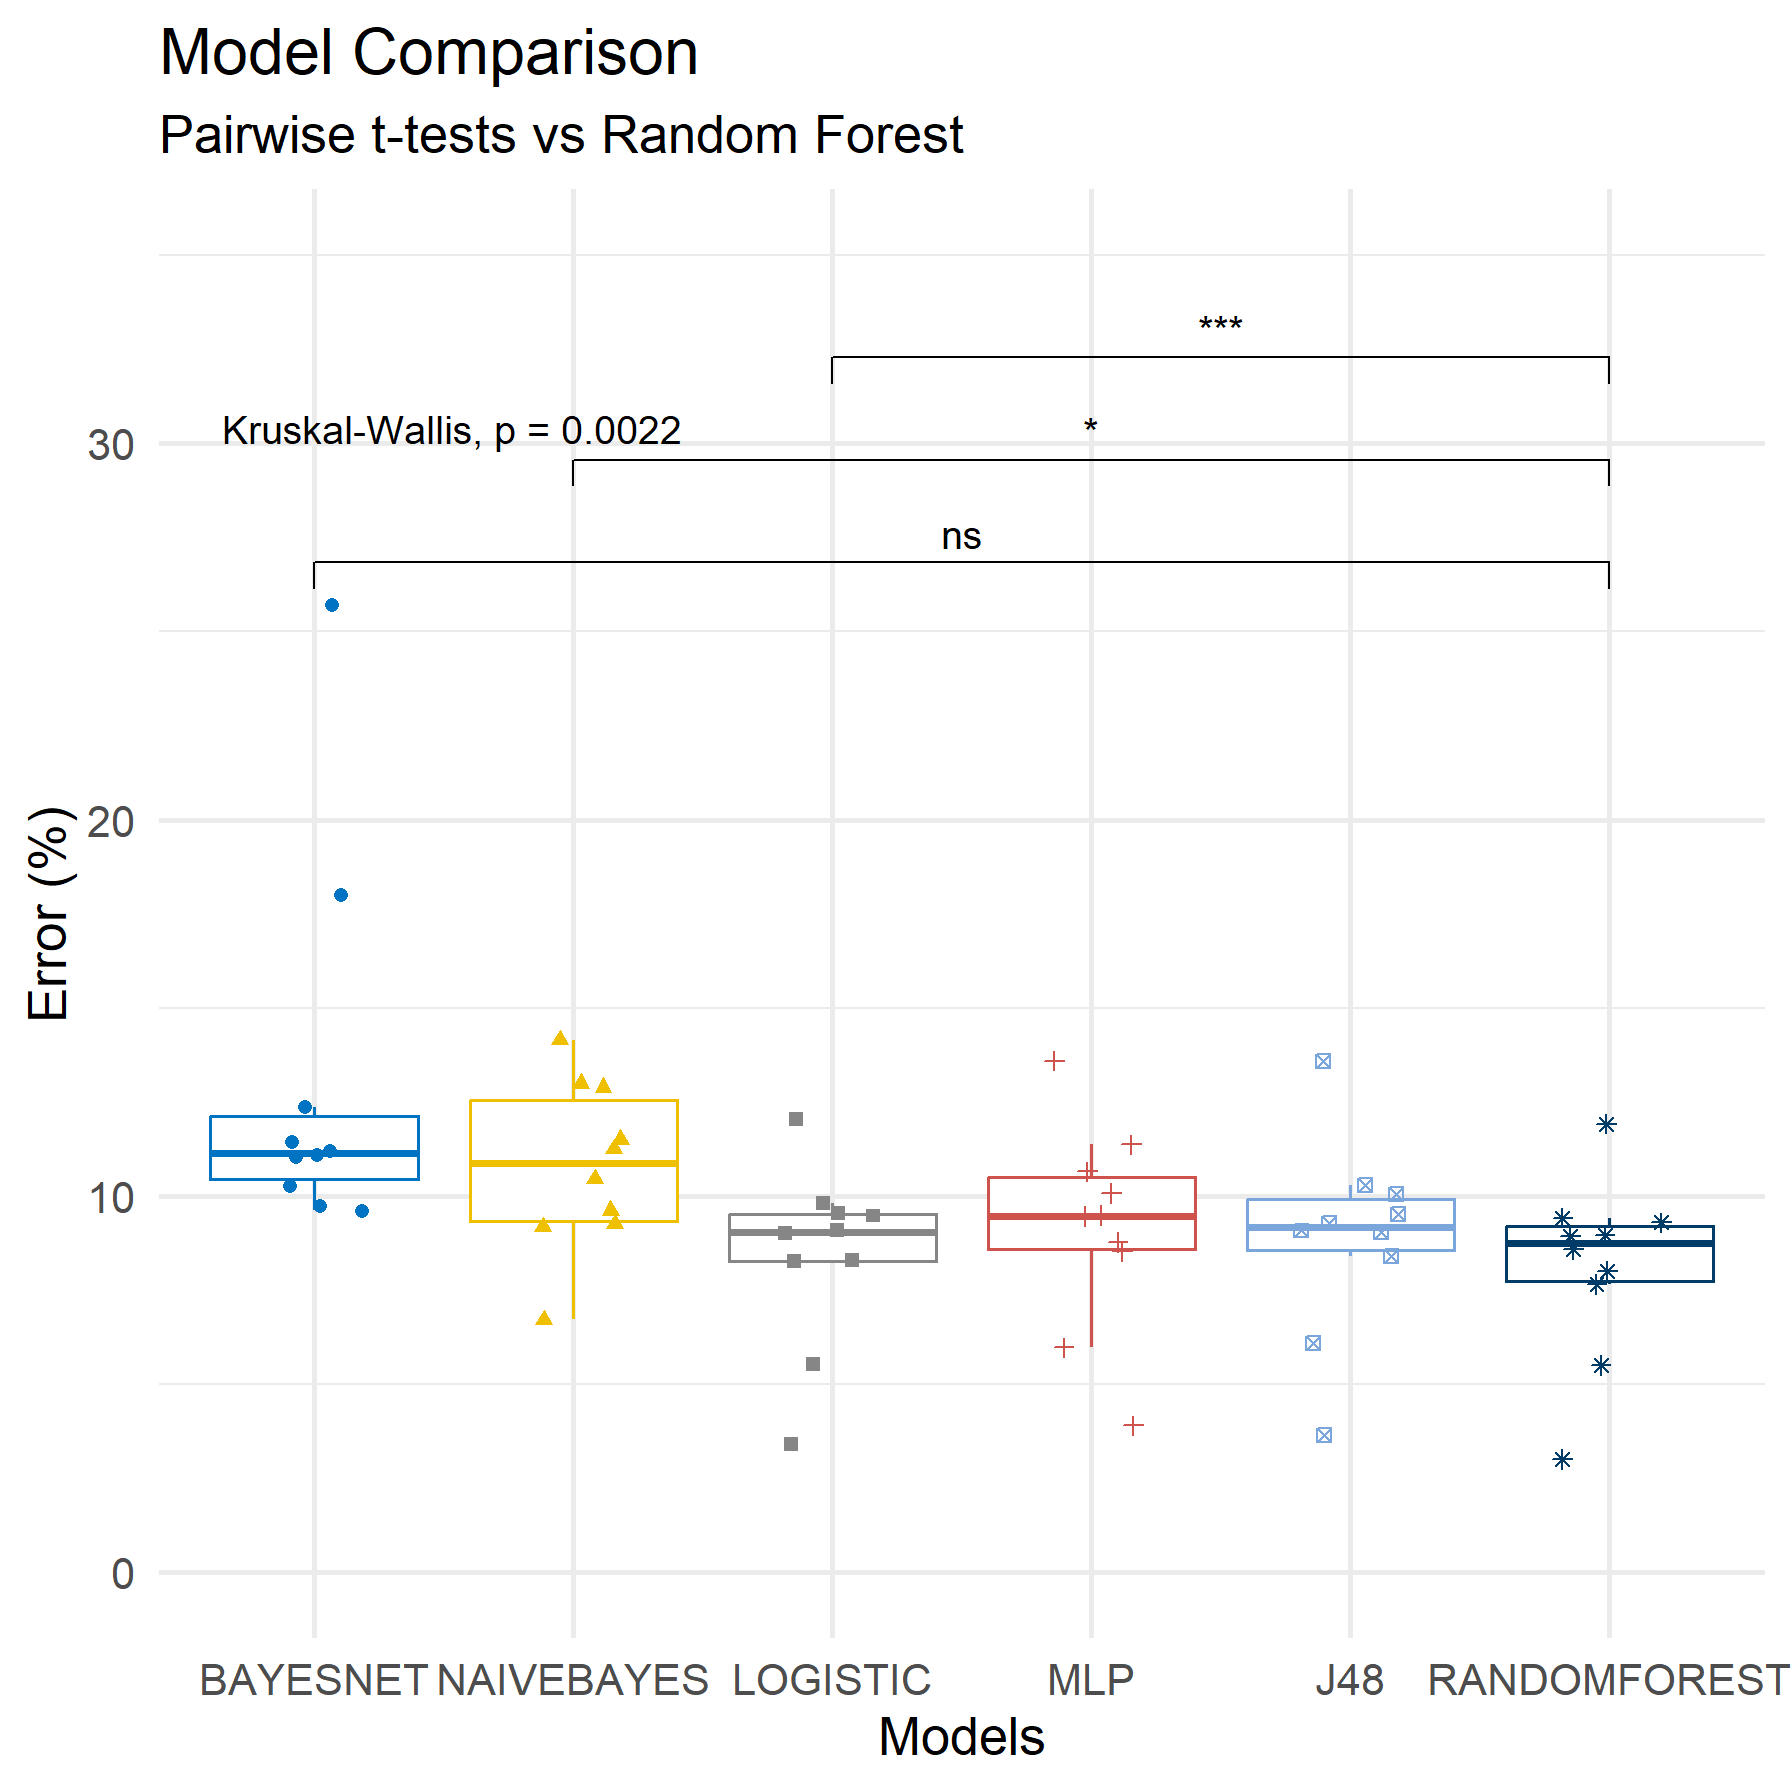
\includegraphics[scale=0.65]{statistic_models_random_forest}
\par\end{centering}
\caption{Statistical comparison between the Random Forest method and the other
machine learning methods.\label{fig:statRandomForest}}

\end{figure}
The results of the Kruskal-Wallis test showed a p-value less than
0.05, leading to the rejection of the null hypothesis. This indicates
that there are statistically significant differences in the error
rates among the models. Based on these findings, the models do not
exhibit uniform performance, with some performing better or worse
than others. Specifically, the \textquotedbl RANDOMFOREST\textquotedbl{}
model was compared to all other models and demonstrated superior performance. 

\section{Conclusions\label{sec:Conclusions}}

A series of machine learning methods was applied on datasets involving
forest fires for the Greece. These datasets covered a period of ten
years, starting from 2014. These methods were obtained from the WEKA
machine learning tool, which is freely available for any operating
system. These methods cover a wide range of machine learning techniques
from different domains. The purpose of this study was to identify
the duration of forest fires and three cases of forest fires were
studied in this research work: forest fires of limited duration, forest
fires of medium duration and forest fires of long duration. Estimating
the duration of a fire is an important factor, as it can be used to
estimate the size of the impending disaster as well as the resources
required to extinguish it. Most of the machine learning techniques
used achieved significantly low error values for each year of experimental
data. On average, these classification error values are in the range
of 8-13\% with the Random Forest technique achieving the lowest value.
The present work could be extended in the future in various research
directions, such as: 
\begin{enumerate}
\item Incorporation of more machine learning methods from the relevant literature.
\item Use feature selection or construction techniques from recent literature
to identify the most important factors influencing the classification
process.
\item Usage of methods that create classification rules, in order to discover
any hidden relationships between the data and the classes of the datasets.
\item Usage of data that also includes meteorological data, in order to
identify a possible correlation of the categories with the meteorological
conditions that prevailed at the time of the fire.
\item Parallel programming techniques may be incorporated to speed up the
optimization process, such as MPI  \citep{MPI} or the OpenMP library
\citep{OPENMP}.
\end{enumerate}
\vspace{6pt}


\authorcontributions{C.K., V.C. and I.G.T. conceived of the idea and the methodology,
and C.K. and V.C. implemented the corresponding software. C.K. conducted
the experiments, employing objective functions as test cases, and
provided the comparative experiments. A.S. performed the necessary
statistical tests. All authors have read and agreed to the published
version of the manuscript.}

\funding{This research received no external funding.}

\institutionalreview{Not applicable.}

\informedconsent{Not applicable. }

\dataavailability{Not applicable. }

\acknowledgments{This research has been financed by the European Union: Next Generation
EU through the Program Greece 2.0 National Recovery and Resilience
Plan, under the call RESEARCH--CREATE--INNOVATE, project name “iCREW:
Intelligent small craft simulator for advanced crew training using
Virtual Reality techniques” (project code: TAEDK-06195).}

\conflictsofinterest{The authors declare no conflicts of interest.}

\begin{adjustwidth}{-\extralength}{0cm}{}

\reftitle{References}
\begin{thebibliography}{999}
\bibitem{forest1}Z. Qiang, E.Z. Meka, R.C. Anderson, Y. Kakabadse,
Forests nature at your service. UNEP report. The magazine of the United
Nations Environment Program, 2011.

\bibitem{forest2}A.S. Mori, K.P. Lertzman, L. Gustafsson, Biodiversity
and ecosystem services in forest ecosystems: a research agenda for
applied forest ecology, Journal of Applied Ecology \textbf{54}, pp.
12-27, 2017.

\bibitem{fire1}B.J. Stocks, Mason, J. A., Todd, J. B., Bosch, E.
M., Wotton, B. M., Amiro, B. D., ... \& Skinner, W. R. (2002). Large
forest fires in Canada, 1959--1997. Journal of Geophysical Research:
Atmospheres, 107(D1), FFR-5.

\bibitem{fire2}M.D. Flannigan, B.D. Amiro, K.A. Logan, B.J. Stocks,
B.M. Wotton, Forest fires and climate change in the 21 st century.
Mitigation and adaptation strategies for global change \textbf{11},
pp. 847-859, 2006.

\bibitem{fire3}O. Sahar, Wildfires in Algeria: problems and challenges.
IFOREST \textbf{8}, pp. 818--826, 2015.

\bibitem{fire_eco1}G. Certini, Effects of fire on properties of forest
soils: a review, Oecologia \textbf{143}, pp. 1--10, 2005.

\bibitem{fire_eco2}G.R. Van Der Werf, J.T. Randerson, G.J. Collatz,
L. GIGLIO, Carbon emissions from fires in tropical and subtropical
ecosystems. Global Change Biology, 9: 547-562, 2003.

\bibitem{fire_eco3}A.A. Agbeshie, S. Abugre, T. Atta-Darkwa et al,
A review of the effects of forest fire on soil properties, J. For.
Res. \textbf{33}, pp. 1419--1441, 2022. 

\bibitem{fire_econ1}P. Aleksić, M. Krstić , G. Jančić, Forest fi
res - ecological and economic problem in Serbia, Botanica Serbia \textbf{32},
pp. 169-176, 2009.

\bibitem{fire_econ2}D. Wang, D. Guan, S. Zhu. et al, Economic footprint
of California wildfires in 2018, Nat Sustain \textbf{4}, pp. 252--260,
2021.

\bibitem{fire_tourism1}P. W. Hystad, P.C. Keller, Towards a destination
tourism disaster management framework: Long-term lessons from a forest
fire disaster, Tourism Management \textbf{29}, pp. 151-162, 2008.

\bibitem{fire_tourism2}G. Boustras, N. Boukas, Forest fires’ impact
on tourism development: a comparative study of Greece and Cyprus,
Management of Environmental Quality \textbf{24}, pp. 498-511, 2013.

\bibitem{fire_tourism3}V. Otrachshenko, L.C. Nunes, Fire takes no
vacation: impact of fires on tourism, Environment and Development
Economics \textbf{27}, pp. 86-101, 2022.

\bibitem{fire_health1}N. Sastry, Forest fires, air pollution, and
mortality in Southeast Asia, Demography \textbf{39}, pp. 1--23, 2002.

\bibitem{fire_health2}E. Frankenberg, D. McKee, D. Thomas, Health
consequences of forest fires in Indonesia, Demography \textbf{42},
pp. 109--129, 2005.

\bibitem{fire_health3}D. Bowman, G. Williamson, J. Abatzoglou. et
al, Human exposure and sensitivity to globally extreme wildfire events,
Nat Ecol Evol \textbf{1}, 0058, 2017. 

\bibitem{fire_stat1}M. Zhong, W. Fan, T. Liu, P. Li, Statistical
analysis on current status of China forest fire safety, Fire Safety
Journal \textbf{38}, pp. 257-269, 2003.

\bibitem{fire_stat2}D. Avila-Flores, M. Pompa-Garcia, X. Antonio-Nemiga.
et al., Driving factors for forest fire occurrence in Durango State
of Mexico: A geospatial perspective, Chin. Geogr. Sci. \textbf{20},
pp. 491--497, 2010.

\bibitem{fire_stat3}R. Lovreglio, V. Leone, P. Giaquinto, A. Notarnicola,
Wildfire cause analysis: four case-studies in southern Italy. iForest
\textbf{3}, pp. 8-15, 2010.

\bibitem{fire_monitor1}D. W. Casbeer, R. W. Beard, T. W. McLain,
Sai-Ming Li and R. K. Mehra, \textquotedbl Forest fire monitoring
with multiple small UAVs,\textquotedbl{} Proceedings of the 2005,
American Control Conference, 2005., Portland, OR, USA, 2005, pp. 3530-3535
vol. 5, doi: 10.1109/ACC.2005.1470520.

\bibitem{fire_monitor2}Guozhu Wang, J. Zhang, Wenbin Li, Dongxu Cui
and Ye Jing, \textquotedbl A forest fire monitoring system based
on GPRS and ZigBee wireless sensor network,\textquotedbl{} 2010 5th
IEEE Conference on Industrial Electronics and Applications, Taichung,
2010, pp. 1859-1862, doi: 10.1109/ICIEA.2010.5515417.

\bibitem{fire_monitor3}M. Stula, D. Krstinic, L. Seric, Intelligent
forest fire monitoring system, Inf Syst Front \textbf{14}, pp. 725--739,
2012. 

\bibitem{fire_monitor4}L. Merino, E. Caballero, J.R. Martínez-de-Dios
al., An Unmanned Aircraft System for Automatic Forest Fire Monitoring
and Measurement, J Intell Robot Syst \textbf{65}, pp. 533--548, 2012. 

\bibitem{fire_monitor5}Y.E. Aslan, I. Korpeoglu, Ö. Ulusoy, A framework
for use of wireless sensor networks in forest fire detection and monitoring,
Computers, Environment and Urban Systems \textbf{36}, pp. 614-625,
2012.

\bibitem{fire_monitor6}M.Á. Serna, R. Casado, A. Bermúdez, N. Pereira,
S. Tennina, Distributed Forest Fire Monitoring Using Wireless Sensor
Networks, International Journal of Distributed Sensor Networks \textbf{11},
10, 2015.

\bibitem{fire_area_class}S. Dwiasnati, Y. Devianto, Classification
of forest fire areas using machine learning algorithm, World Journal
of Advanced Engineering Technology and Sciences, \textbf{3}, pp. 008-015,
2021.

\bibitem{fire_prediction_china}Y. Pang, Y. Li, Z. Feng, Z. Feng,
Z. Zhao, S. Chen, H. Zhang, Forest Fire Occurrence Prediction in China
Based on Machine Learning Methods, Remote Sensing \textbf{14}, 5546,
2022.

\bibitem{fire_detection_dampage}U. Dampage, L. Bandaranayake, R.
Wanasinghe et al, Forest fire detection system using wireless sensor
networks and machine learning, Sci Rep \textbf{12}, 46, 2022. 

\bibitem{fire_parallel_svm}K.R. Singh, K.P. Neethu, K. Madhurekaa,
A. Harita, P. Mohan, Parallel SVM model for forest fire prediction,
Soft Computing Letters \textbf{3}, 100014, 2021.

\bibitem{fire_ml_survey}F. Abid, A survey of machine learning algorithms
based forest fires prediction and detection systems, Fire technology
\textbf{57}, pp. 559-590, 2021.

\bibitem{fire_risk}Y. Shao, Z. Feng, L. Sun, X. Yang, Y. Li, B. Xu,
Y. Chen, Mapping China’s Forest Fire Risks with Machine Learning,
Forests \textbf{13}, 856, 2022.

\bibitem{fire_image1}J. Vicente, P. Guillemant, An image processing
technique for automatically detecting forest fire, International Journal
of Thermal Sciences \textbf{41}, pp. 1113-1120, 2002.

\bibitem{fire_image2}Q. Yan, P. Bo, Z. Juanjuan, Forest Fire Image
Intelligent Recognition based on the Neural Network. Journal of Multimedia
\textbf{9}, pp. 469-475, 2014.

\bibitem{fire_image4}Mahmoud, Mubarak A. I., Ren, Honge, Forest Fire
Detection Using a Rule-Based Image Processing Algorithm and Temporal
Variation, Mathematical Problems in Engineering, 2018, 7612487, 8
pages, 2018. 

\bibitem{fire_image5}Y. Wang, L. Dang, J. Ren, Forest fire image
recognition based on convolutional neural network, Journal of Algorithms
\& Computational Technology \textbf{13}, 2019.

\bibitem{fire_image6}Z. Jiao, Y. Zhang, J. Xin, Y. Yi, D. Liu and
H. Liu, \textquotedbl Forest Fire Detection with Color Features and
Wavelet Analysis Based on Aerial Imagery,\textquotedbl{} 2018 Chinese
Automation Congress (CAC), Xi'an, China, 2018, pp. 2206-2211, doi:
10.1109/CAC.2018.8623473.

\bibitem{fire_duration1}H. Liang, M. Zhang, H. Wang, A Neural Network
Model for Wildfire Scale Prediction Using Meteorological Factors,
IEEE Access \textbf{7}, pp. 176746-176755, 2019.

\bibitem{fire_duration2}U. KC, J. Aryal, J. Hilton, S. Garg, A Surrogate
Model for Rapidly Assessing the Size of a Wildfire over Time, Fire
\textbf{4}, 20, 2021.

\bibitem{fire_duration3}D.D. Xi, C.B. Dean, S.W. Taylor, Modeling
the duration and size of wildfires using joint mixture models. Environmetrics
\textbf{32}, e2685, 2021.

\bibitem{log_norm}H.M. Hammouri, R.T. Sabo, R. Alsaadawi, K.A. Kheirallah,
Handling Skewed Data: A Comparison of Two Popular Methods. Applied
Sciences \textbf{10}, 6247, 2020.

\bibitem{bayes_net1}Ben-Gal, I. (2008). Bayesian Networks. In Encyclopedia
of Statistics in Quality and Reliability (eds F. Ruggeri, R.S. Kenett
and F.W. Faltin).

\bibitem{bayes_net2} Koski, T., \& Noble, J. (2011). Bayesian networks:
an introduction. John Wiley \& Sons.

\bibitem{bayes_net_expression}N. Friedman, M. Linial, I. Nachman,
D. Pe'er, Using Bayesian networks to analyze expression data, In:
Proceedings of the fourth annual international conference on Computational
molecular biology, pp. 127-135, 2000.

\bibitem{bayes_net_fault}B. Cai, L. Huang, M. Xie, Bayesian Networks
in Fault Diagnosis, IEEE Transactions on Industrial Informatics \textbf{13},
pp. 2227-2240, 2017.

\bibitem{bayes_net_environ}D.N. Barton, S. Kuikka, O. Varis, L. Uusitalo,
H.J. Henriksen, M. Borsuk, A. de la Hera, R. Farmani, S. Johnson,
J.D. Linnell, Bayesian networks in environmental and resource management.
Integr Environ Assess Manag, \textbf{8}, pp. 418-429, 2012.

\bibitem{bayes_net_fire_cause}V. Sevinc, O. Kucuk, M. Goltas, A Bayesian
network model for prediction and analysis of possible forest fire
causes. Forest Ecology and Management \textbf{457}, 117723, 2020.

\bibitem{bayes_net_cascade}F. Chen, H. Jia, E. Du, Y. Chen, L. Wang,
Modeling of the cascading impacts of drought and forest fire based
on a Bayesian network, International Journal of Disaster Risk Reduction
\textbf{111}, 104716,2024.

\bibitem{bayes_net_video}B. Kim, J. Lee, A Bayesian network-based
information fusion combined with DNNs for robust video fire detection.
Applied Sciences \textbf{11}, 7624, 2021.

\bibitem{naive_bayes1}Bayes, T. (1968). Naive bayes classifier. Article
Sources and Contributors, 1-9.

\bibitem{naive_bayes2}G.I. Webb, E. Keogh, R. Miikkulainen, Naïve
Bayes, Encyclopedia of machine learning \textbf{15}, pp. 713-714,
2010.

\bibitem{naive_bayes_document}S.L. Ting, W.H. Ip, A.H. Tsang, Is
Naive Bayes a good classifier for document classification, International
Journal of Software Engineering and Its Applications \textbf{5}, pp.
37-46, 2011.

\bibitem{naive_bayes_traffic}H. Chen, S. Hu, R. Hua, et al, Improved
naive Bayes classification algorithm for traffic risk management,
EURASIP J. Adv. Signal Process. 2021, 30, 2021.

\bibitem{naive_bayes_network}M. Panda, M.R. Patra, Network intrusion
detection using naive bayes. International journal of computer science
and network security \textbf{7}, pp. 258-263, 2007.

\bibitem{naive_bayes_fire1}A. Andi Nugroho, I. Iwan, K. Iroh Nur
Azizah, F. Hakim Raswa, Peatland Forest Fire Prevention Using Wireless
Sensor Network Based on Naïve Bayes Classifier, KnE Social Sciences
\textbf{3}, pp. 20--34, 2019.

\bibitem{naive_bayes_fire2}M. Zainul, E. Minggu, Classification of
Hotspots Causing Forest and Land Fires Using the Naive Bayes Algorithm,
Interdisciplinary Social Studies \textbf{1}, pp. 555-567, 2022.

\bibitem{naive_bayes_fire3}I.M.K. Karo, S.N. Amalia, D. Septiana,
Wildfires Classification Using Feature Selection with K-NN, Naïve
Bayes, and ID3 Algorithms, Journal of Software Engineering, Information
and Communication Technology (SEICT) \textbf{3}, pp. 15-24, 2022.

\bibitem{naive_bayes_fire4}L. Shu, H. Zhang, Y. You, Y. Cui, W. Chen,
Towards fire prediction accuracy enhancements by leveraging an improved
naïve bayes algorithm, Symmetry \textbf{13}, 530, 2021.

\bibitem{logistic_def}S. Sperandei, Understanding logistic regression
analysis, Biochemia medica \textbf{24}, pp. 12-18, 2014.

\bibitem{logistic_education}A.F. Cabrera, Logistic regression analysis
in higher education: An applied perspective, Higher education: Handbook
of theory and research \textbf{10}, pp. 225-256, 1994.

\bibitem{logistic_customer}C. Lawson, D.C. Montgomery, Logistic Regression
Analysis of Customer Satisfaction Data, Qual. Reliab. Engng. Int.
\textbf{22}, pp. 971-984, 2006.

\bibitem{logistic_urban}Zhiyong Hu and C.P. Lo, Modeling urban growth
in Atlanta using logistic regression, Computers, Environment and Urban
Systems \textbf{31}, pp. 667-688, 2007.

\bibitem{logistic_fire1}L. Vilar del Hoyo, M.P. Martín Isabel, F.J.
Martínez Vega, Logistic regression models for human-caused wildfire
risk estimation: analysing the effect of the spatial accuracy in fire
occurrence data, Eur J Forest Res \textbf{130}, pp. 983--996, 2011. 

\bibitem{logistic_fire2}P.P. de Bem, O.A. de Carvalho Júnior, E.A.T.
Matricardi, R.F. Guimarães, R.A.T. Gomes, Predicting wildfire vulnerability
using logistic regression and artificial neural networks: a case study
in Brazil’s Federal District. International journal of wildland fire
\textbf{28}, pp. 35-45, 2018.

\bibitem{logistic_fire3}Eufrásio João Sozinho Nhongo, Denise Cybis
Fontana, Laurindo Antonio Guasselli and Carolina Bremm, Probabilistic
modelling of wildfire occurrence based on logistic regression, Niassa
Reserve, Mozambique, Geomatics, Natural Hazards and Risk \textbf{10},
pp. 1772-{}-1792, 2019.

\bibitem{logistic_fire4}W. Peng, Y. Wei, G. Chen, G. Lu, Q. Ye, R.
Ding, P. Hu, Z. Cheng, Analysis of Wildfire Danger Level Using Logistic
Regression Model in Sichuan Province, China. Forests \textbf{14},
2352, 2023.

\bibitem{nn1}C. Bishop, Neural Networks for Pattern Recognition,
Oxford University Press, 1995.

\bibitem{nn2}G. Cybenko, Approximation by superpositions of a sigmoidal
function, Mathematics of Control Signals and Systems \textbf{2}, pp.
303-314, 1989.

\bibitem{nnphysics1}P. Baldi, K. Cranmer, T. Faucett et al, Parameterized
neural networks for high-energy physics, Eur. Phys. J. C \textbf{76},
2016.

\bibitem{nnphysics2}J. J. Valdas and G. Bonham-Carter, Time dependent
neural network models for detecting changes of state in complex processes:
Applications in earth sciences and astronomy, Neural Networks \textbf{19},
pp. 196-207, 2006

\bibitem{nnphysics3}G. Carleo,M. Troyer, Solving the quantum many-body
problem with artificial neural networks, Science \textbf{355}, pp.
602-606, 2017.

\bibitem{nnde1}Y. Shirvany, M. Hayati, R. Moradian, Multilayer perceptron
neural networks with novel unsupervised training method for numerical
solution of the partial differential equations, Applied Soft Computing
\textbf{9}, pp. 20-29, 2009.

\bibitem{nnde2}A. Malek, R. Shekari Beidokhti, Numerical solution
for high order differential equations using a hybrid neural network---Optimization
method, Applied Mathematics and Computation \textbf{183}, pp. 260-271,
2006.

\bibitem{nn_solar}A. Kumar Yadav, S.S. Chandel, Solar radiation prediction
using Artificial Neural Network techniques: A review, Renewable and
Sustainable Energy Reviews \textbf{33}, pp. 772-781, 2014.

\bibitem{nnagr1}A. Topuz, Predicting moisture content of agricultural
products using artificial neural networks, Advances in Engineering
Software \textbf{41}, pp. 464-470, 2010.

\bibitem{nnagr2}A. Escamilla-García, G.M. Soto-Zarazúa, M. Toledano-Ayala,
E. Rivas-Araiza, A. Gastélum-Barrios, Abraham,Applications of Artificial
Neural Networks in Greenhouse Technology and Overview for Smart Agriculture
Development, Applied Sciences \textbf{10}, Article number 3835, 2020.

\bibitem{nnchem1}Lin Shen, Jingheng Wu, and Weitao Yang, Multiscale
Quantum Mechanics/Molecular Mechanics Simulations with Neural Networks,
Journal of Chemical Theory and Computation \textbf{12}, pp. 4934-4946,
2016.

\bibitem{nnchem2}Sergei Manzhos, Richard Dawes, Tucker Carrington,
Neural network‐based approaches for building high dimensional and
quantum dynamics‐friendly potential energy surfaces, Int. J. Quantum
Chem. \textbf{115}, pp. 1012-1020, 2015.

\bibitem{nnchem3}Jennifer N. Wei, David Duvenaud, and Alán Aspuru-Guzik,
Neural Networks for the Prediction of Organic Chemistry Reactions,
ACS Central Science \textbf{2}, pp. 725-732, 2016.

\bibitem{nn_wind}G. Li, J. Shi, On comparing three artificial neural
networks for wind speed forecasting, Applied Energy \textbf{87}, pp.
2313-2320, 2010.

\bibitem{nnecon1}Lukas Falat and Lucia Pancikova, Quantitative Modelling
in Economics with Advanced Artificial Neural Networks, Procedia Economics
and Finance \textbf{34}, pp. 194-201, 2015.

\bibitem{nnecon2}Mohammad Namazi, Ahmad Shokrolahi, Mohammad Sadeghzadeh
Maharluie, Detecting and ranking cash flow risk factors via artificial
neural networks technique, Journal of Business Research \textbf{69},
pp. 1801-1806, 2016.

\bibitem{nncecon3}G. Tkacz, Neural network forecasting of Canadian
GDP growth, International Journal of Forecasting \textbf{17}, pp.
57-69, 2001.

\bibitem{nnmed1}Igor I. Baskin, David Winkler and Igor V. Tetko,
A renaissance of neural networks in drug discovery, Expert Opinion
on Drug Discovery \textbf{11}, pp. 785-795, 2016.

\bibitem{nnmed2}Ronadl Bartzatt, Prediction of Novel Anti-Ebola Virus
Compounds Utilizing Artificial Neural Network (ANN), Chemistry Faculty
Publications \textbf{49}, pp. 16-34, 2018.

\bibitem{nn_fire1}F. M. A. Hossain, Y. Zhang, C. Yuan and C. -Y.
Su, \textquotedbl Wildfire Flame and Smoke Detection Using Static
Image Features and Artificial Neural Network,\textquotedbl{} 2019
1st International Conference on Industrial Artificial Intelligence
(IAI), Shenyang, China, 2019, pp. 1-6, doi: 10.1109/ICIAI.2019.8850811.

\bibitem{nn_fire2}S. Lall and B. Mathibela, \textquotedbl The application
of artificial neural networks for wildfire risk prediction,\textquotedbl{}
2016 International Conference on Robotics and Automation for Humanitarian
Applications (RAHA), Amritapuri, India, 2016, pp. 1-6, doi: 10.1109/RAHA.2016.7931880.

\bibitem{nn_fire3}Y. O. Sayad, H. Mousannif, H. Al Moatassime, Predictive
modeling of wildfires: A new dataset and machine learning approach,
Fire Safety Journal \textbf{104}, pp. 130-146, 2019.

\bibitem{nn_fire4}H. Liang, M. Zhang, H. Wang, A Neural Network Model
for Wildfire Scale Prediction Using Meteorological Factors, IEEE Access
\textbf{7}, pp. 176746-176755, 2019.

\bibitem{nn_fire5}K. Gao, Z. Feng, S. Wang, Using multilayer perceptron
to predict forest fires in jiangxi province, southeast china, Discrete
Dynamics in Nature and Society \textbf{1}, 6930812, 2022.

\bibitem{j48_1}N. Bhargava, G. Sharma, R. Bhargava, M. Mathuria,
Decision tree analysis on j48 algorithm for data mining. Proceedings
of international journal of advanced research in computer science
and software engineering \textbf{3}, 2013.

\bibitem{j48_diabetes}G. Kaur, A. Chhabra, Improved J48 classification
algorithm for the prediction of diabetes, International journal of
computer applications \textbf{98}, 22, 2014.

\bibitem{j48_network}S. Sahu, B.M. Mehtre, Network intrusion detection
system using J48 Decision Tree, In: 2015 International Conference
on Advances in Computing, Communications and Informatics (ICACCI),
pp. 2023-2026, 2015.

\bibitem{j48_criminal}N.N. Sakhare, S.A. Joshi, Classification of
criminal data using J48-Decision Tree algorithm. Int. J. Data Warehous.
Min \textbf{4}, pp. 167-171, 2015.

\bibitem{j48_finger}S.F. Abdullah, A.F.N.A. Rahman, Z.A. Abas, W.H.M.
Saad, Fingerprint gender classification using univariate decision
tree (j48), International Journal of Advanced Computer Science and
Applications \textbf{7}, 2016.

\bibitem{j48_fake}Jehad, R., \& Yousif, S. A. (2020). Fake news classification
using random forest and decision tree (j48). Al-Nahrain Journal of
Science, 23(4), 49-55.

\bibitem{j48_forest1}D. Stojanova, P. Panov, A. Kobler, S. Džeroski,
K. Taškova, Learning to predict forest fires with different data mining
techniques. In Conference on data mining and data warehouses (SiKDD
2006), Ljubljana, Slovenia, pp. 255-258, 2006.

\bibitem{j48_forest2}F. Abid, N. Izeboudjen, Predicting forest fire
in algeria using data mining techniques: Case study of the decision
tree algorithm. In Advanced Intelligent Systems for Sustainable Development
(AI2SD’2019) Volume 4-Advanced Intelligent Systems for Applied Computing
Sciences (pp. 363-370). Springer International Publishing, 2020.

\bibitem{random_forest1}Breiman, L. (2001). Random forests. Machine
learning, 45, 5-32.

\bibitem{random_forest2}S.J. Rigatti, Random forest, Journal of Insurance
Medicine, 47(1), 31-39, 2017.

\bibitem{random_forest_remote}M. Pal, Random forest classifier for
remote sensing classification. International Journal of Remote Sensing
\textbf{26}, pp. 217--222, 2005.

\bibitem{random_forest_ecology}D.R. Cutler, T.C. Edwards, K.H. Beard,
A. Cutler, K.T. Hess, J. Gibson, J.J. Lawler, random forests for classification
in ecology. Ecology \textbf{88}, pp. 2783-2792, 2007.

\bibitem{random_forest_bio}Qi, Y. (2012). Random Forest for Bioinformatics.
In: Zhang, C., Ma, Y. (eds) Ensemble Machine Learning. Springer, New
York, NY. https://doi.org/10.1007/978-1-4419-9326-7\_11

\bibitem{random_forest_text}B. Xu, X. Guo, Y. Ye, J. Cheng, An improved
random forest classifier for text categorization. J. Comput., \textbf{7},
pp. 2913-2920, 2012.

\bibitem{random_forest_network}N. Farnaaz, M.A. Jabbar, Random Forest
Modeling for Network Intrusion Detection System, Procedia Computer
Science \textbf{89}, pp. 213-217, 2016.

\bibitem{random_forest_fire1}A. L. Latifah, A. Shabrina, I. N. Wahyuni,
R. Sadikin, Evaluation of Random Forest model for forest fire prediction
based on climatology over Borneo, In: 2019 International Conference
on Computer, Control, Informatics and its Applications (IC3INA), Tangerang,
Indonesia, pp. 4-8, 2019.

\bibitem{random_forest_fire2}A. Malik, M.R. Rao, N. Puppala, P. Koouri,
V.A.K. Thota, Q. Liu, S. Chiao, J. Gao, Data-Driven Wildfire Risk
Prediction in Northern California. Atmosphere, \textbf{12}, 109, 2021. 

\bibitem{random_forest_fire3}C. Gao, H. Lin, H. Hu, Forest fire risk
prediction based on random forest and backpropagation neural network
of Heihe area in Heilongjiang province, China, Forests \textbf{14},
170, 2023.

\bibitem{bpnn1}D.E. Rumelhart, G.E. Hinton and R.J. Williams, Learning
representations by back-propagating errors, Nature \textbf{323}, pp.
533 - 536 , 1986.

\bibitem{weka_main}M. Hall, F. Frank, G. Holmes, B. Pfahringer, P.
Reutemann, I.H. Witten, The WEKA data mining software: an update.
ACM SIGKDD explorations newsletter \textbf{11}, pp. 10-18, 2009.

\bibitem{weka_education1}S.B. Aher, L.M.R.J. Lobo, Data mining in
educational system using weka. In International conference on emerging
technology trends, Foundation of Computer Science \textbf{3}, pp.
20-25, 2011.

\bibitem{weka_education2}S. Hussain, N.A. Dahan, F.M. Ba-Alwib, N.
Ribata, Educational data mining and analysis of students’ academic
performance using WEKA. Indonesian Journal of Electrical Engineering
and Computer Science \textbf{9}, pp. 447-459, 2018.

\bibitem{weka_medical1}A.K. Sigurdardottir, H. Jonsdottir, R. Benediktsson,
Outcomes of educational interventions in type 2 diabetes: WEKA data-mining
analysis. Patient education and counseling \textbf{67}, pp. 21-31,
2007.

\bibitem{weka_medical2}M.N. Amin, A. Habib, Comparison of different
classification techniques using WEKA for hematological data. American
Journal of Engineering Research \textbf{4}, pp. 55-61, 2015.

\bibitem{MPI}Gropp, W.; Lusk, E.; Doss, N.; Skjellum, A. A high-performance,
portable implementation of the MPI message passing interface standard.
Parallel Comput. 1996, 22, 789--828.

\bibitem{OPENMP}Chandra, R. Parallel Programming in OpenMP; Morgan
Kaufmann: Cambridge, MA, USA, 2001.

\end{thebibliography}
%%%%%%%%%%%%%%%%%%%%%%%%%%%%%%%%%%%%%%%%%%
%% for journal Sci
%\reviewreports{\\
%Reviewer 1 comments and authors' response\\
%Reviewer 2 comments and authors' response\\
%Reviewer 3 comments and authors' response
%}
%%%%%%%%%%%%%%%%%%%%%%%%%%%%%%%%%%%%%%%%%%

\PublishersNote{}

\end{adjustwidth}{}
\end{document}
